
%
%   svt_calibrations.tex
%       author: Omar Moreno <omoreno1@ucsc.edu>
%               Per Hansson <phansson@slac.stanford.edu>
%
%

In order to prepare the SVT for real physics data-taking, the SVT was 
calibrated. This involved the extraction of the mean baseline (pedestal),
baseline noise and gain for each of the 12,780 SVT channels. All measurements
were made with the APV25 readout chips configured to their nominal operating
points \cite{Jones:1069892} and all sensors biased to 180 V. The APV25s were
operated in ``mulit-peak'' mode with six samples being readout per trigger.
This, in turn, allowed for the extraction of the $t_0$ and amplitude of the 
signals being read out.

Figure~\ref{fig:pedestal_noise} shows an intensity plot of the pedestals 
along with the readout noise as a function of channel number for a single
hybrid.  The noise was computed by taking the RMS of the gaussian distributed
\begin{figure}[h]
    \begin{center}
    	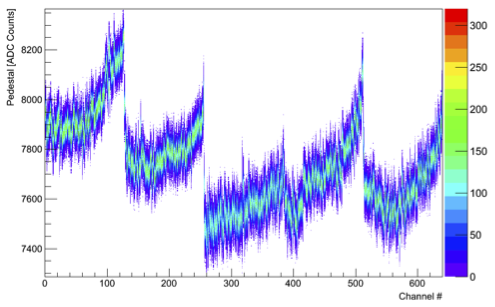
\includegraphics[width=0.45\textwidth]{test2012/svtperformance/baseline}
    	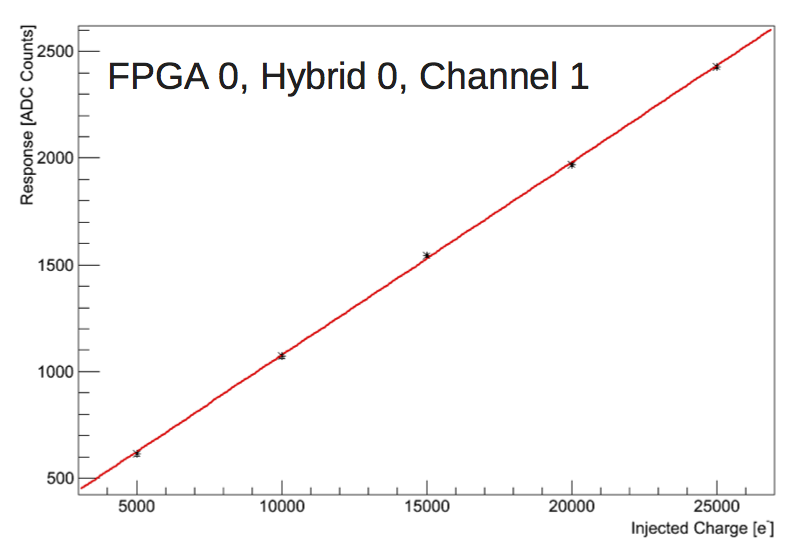
\includegraphics[width=0.45\textwidth]{test2012/svtperformance/gain}
        \caption{Something ... }
%    	\caption{\small{The baseline across a hybrid (left) and the measured response as a function of 
%	                    input charge (right). The overall shifts in the baseline are calibrated out where distinct edges 
%	                    are associated with the five APV25 chips on the hybrid. The gain shows good linearity up to 
%	                    about three $mip$s.} {\color{red}Should we show noise instead of baseline?}}
	\label{fig:pedestal_noise}
    \end{center}
\end{figure}
pedestals for each of the channels and was observed to be consistently within 
[Find number] ADC counts ( electrons).  One observed feature are the large
noise values for the channels lying near the chip edges.  This has also been 
reported by the CMS collaboration and the cause is still under investigation.

%  Need to rewrite this ...
Another important aspect for the characterization of the SVT is the response and the associated 
gain. Using the APV25 internal calibration circuit a known fixed charge was injected into all 
channels of the which allows for an accurate determination of the response and its 
scaling with input charge, shown in Fig.~\ref{fig:baseline_and_gain}. The gain uniformity was 
within the expected range across chips and modules and show good linearity of charge 
depositions up to about 3 $mip$s. 

All reconstructed hits in an event were used to form clusters of energy 
depositions using a nearest neighbor algorithm. Fig.~\ref{fig:cluster_pulse}
shows the mean pulse shape of each of the hits associated with a track as a 
function of time.  
\begin{figure}[h]
	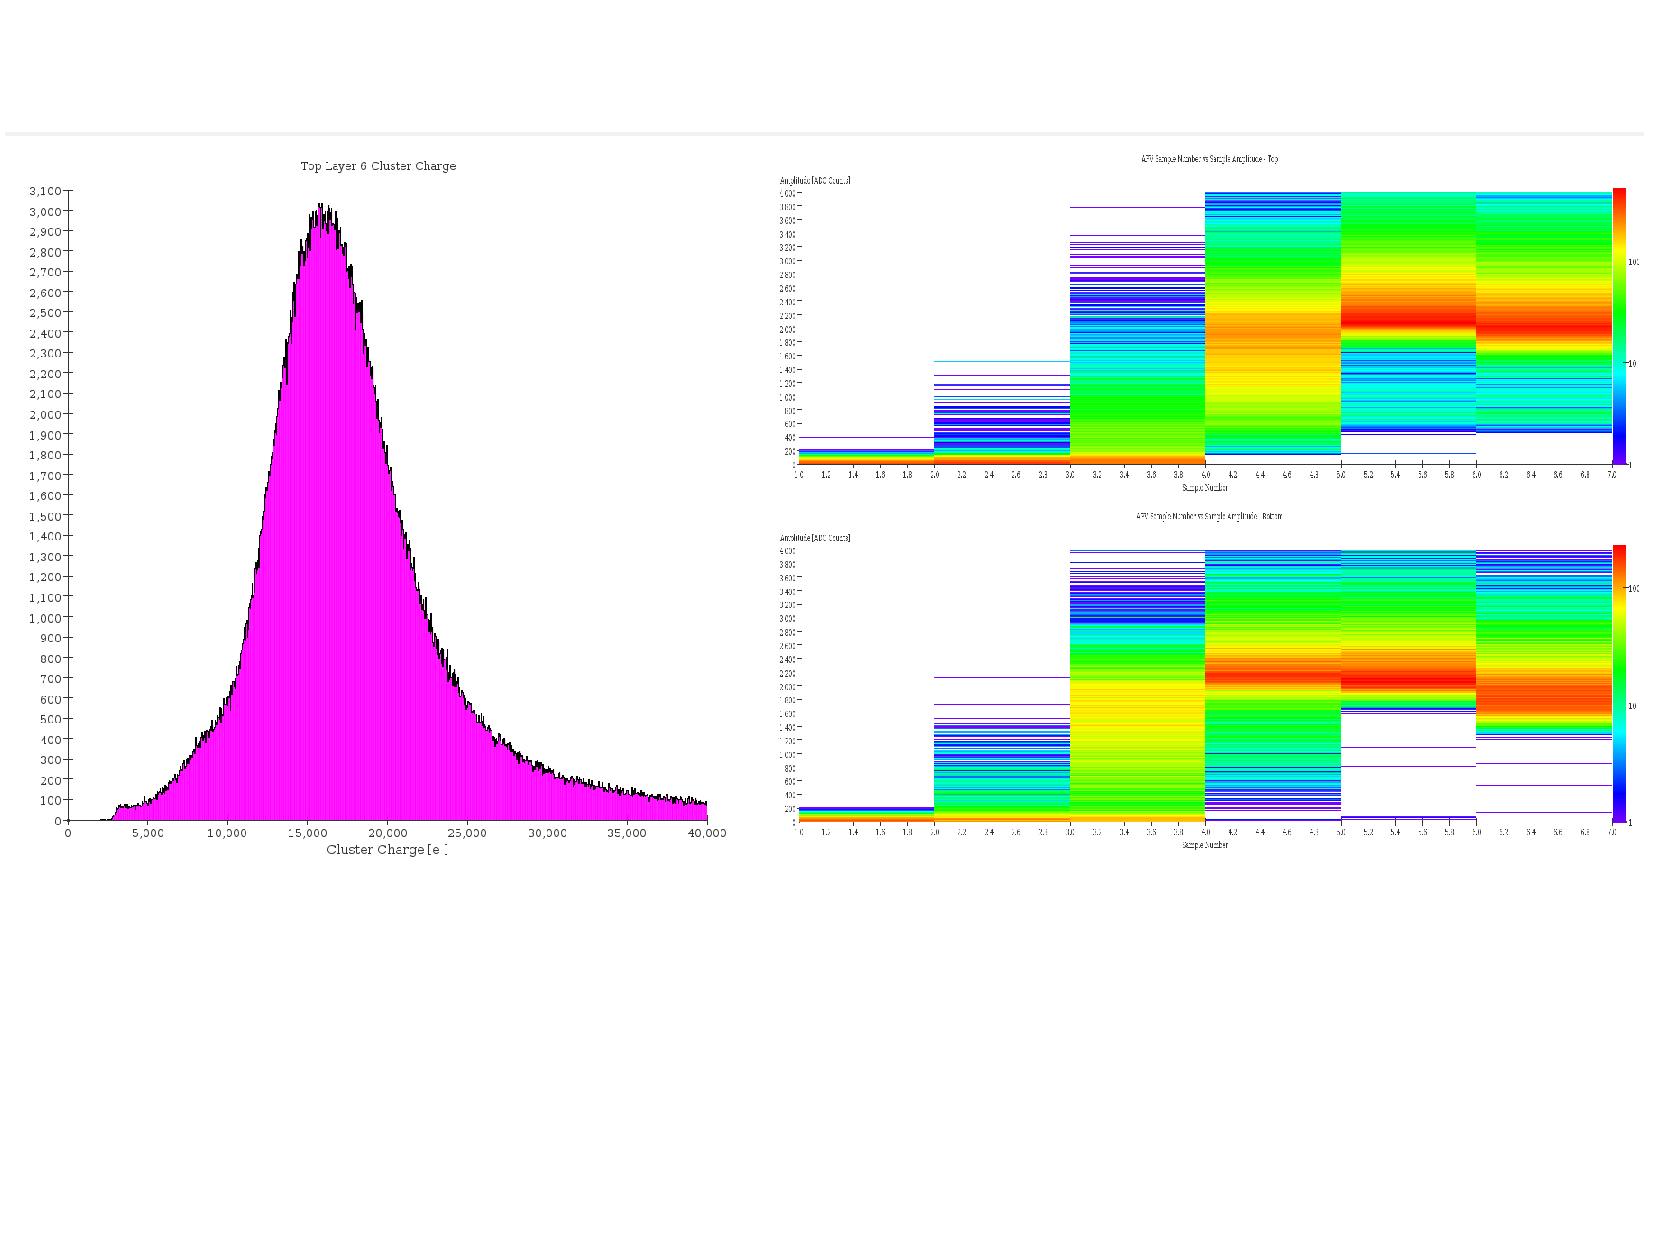
\includegraphics[width=\textwidth]{test2012/svtperformance/pulseshape_and_landau}
    \caption{Something else ...}
%	\caption{\small{The distribution of cluster amplitudes (left) showing the characteristic Landau 
%	shape and the pulse shape from the six samples readout (right) {\color{red} Remove one of the pulse shapes}. }}
	\label{fig:pulseshape}
\end{figure}
% Should this be included? If so, it needs to be rewritten a little better
The figure also demostrates that  the trigger system, described below, is well 
timed in with the tracker. 
Fig.~\ref{fig:cluster_pulse} shows the MIP response to be [Find value] electrons.
Taking the MIP response, the signal to noise ratio was calculated to be 
approximately 25.5 which is well matched to the expected behavior.

\bibliography{svt_calib}
 
